El primer brazo mecánico teleoperado se desarrollo por Raymond Goertz en 1949 y fue llamado \textit{M1}. El objetivo de su desarrollo era proteger del riesgo a los trabajadores mientras se permite la manipulación precisa de materiales o elementos radiactivos. Este es considerado el pionero en aplicar la técnica maestro-esclavo en sistemas de teleoperación. Más concretamente, en la máquina se consideran dos dispositivos diferenciados un brazo \textit{maestro} y otro brazo \textit{esclavo}. El brazo \textit{esclavo} se ubica dentro de un recipiente aislado en su totalidad y el brazo \textit{maestro} se sitúa en una sala de control y es el encargado de ejecutar ordenes que posteriormente el \textit{esclavo} reproducirá sobre el material radioactivo con notable precisión.

En 1951, Goertz diseñó una mejora en este brazo mediante la incorporación de una serie de poleas y cables de acero entre el brazo \textit{maestro} y el brazo \textit{esclavo} que proporcionaba mayor precisión en sus movimientos.\\

Durante el desarrollo de dicho brazo robótico, Goertz estableció uno principios que debía cumplir un brazo de este tipo y que aún se siguen aplicando a los robots quirúrgicos que se utilizan hoy en día. Los principios son los siguientes:

\begin{enumerate}
\item El movimiento del brazo \textit{esclavo} debe tener seis grados de libertad; tres de traslación, tres de rotación y uno de agarre.

\item El movimiento del brazo \textit{esclavo} debe estar acoplado al brazo \textit{maestro}.

\item Dicho acoplamiento debe ser bilateral, es decir, las fuerzas sobre el brazo \textit{esclavo} deben reflejarse en el brazo \textit{maestro} y los desplazamientos de producidos por el brazo \textit{maestro} deben producir el mismo desplazamiento sobre el brazo \textit{esclavo}.

\end{enumerate}


Seguidamente se muestra una imagen donde se puede observar el brazo robótico de Goertz descrito anteriormente.



\begin{figure}[H]
\begin{center}
  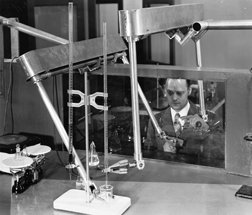
\includegraphics[width=0.5\textwidth]{./EtapaPrimeriza/imagenes/brazo.jpg}
  \caption{Brazo robótico de Goertz (\href{https://en.wikipedia.org/wiki/Raymond\_Goertz\#/media/File:Apf1-06395t.jpg} {Wikipedia})}
  \label{brazo}
\end{center}
\end{figure}
